\section{Modelando la m\'etrica}
\subsection{Fundamentos}
El acento m'etrico es una caracter'istica inherente a la m'usica tonal; cualquier pieza musical se enmarca en una estructura 
(posiblemente ambigua) de beats fuertes y d'ebiles. Si bien 'esta existe solamente en la mente del escucha, las reglas para inferirla son culturalmente conocidas, 
y colocan al acento m'etrico como un elemento importante dentro del lenguaje musical. La estructura m'etrica ayuda a medir el tiempo permitiendo a un interprete 
reproducir y a un oyente reconocer un cierto conjunto de relaci'ones temporales. Esta estructura da contexto para interpretar la r'itmica,  
donde por r'itmica se refiere a un grupo de al menos dos eventos musicales en donde hay uno acentuado con respecto al resto \cite{CooperMeyer60}.
Es por esto que un patr'on temporal as'i descripto es interpretado de forma distinta seg'un el contexto m'etrico\footnote{como hago para explicar en dos palabras que es contexto metrico? no se entiende de este parrafo que es un patron de beats fuertes y debiles?} donde sea escuchado. 

 \comment{Mencionar la ``localidad'' de los acentos metricos (no se perciben a niveles altos)}
Siguiendo la teor\'ia de Lerdahl y Jackendoff el acento m'etrico es una construcci'on que si bien es jer'arquica, lo niveles altos no son percibidos, puesto
que en esos niveles entran en juego los acentos estructurales y los acentos fenom'enicos. De esta forma se habla de la \emph{localidad} de los acentos m'etricos: 
s'olo se perciben a niveles bajos en la jerarqu'ia\footnote{meter en la intro la nocion de nivel alto $\leftrightarrow$ timespan largo}. 

 \comment{Definir el paso del tiempo como saltos entre las clases de equivalencia}
La estructura m'etrica permite organizar los distintos puntos en el tiempo en clases de 
equivalencia de forma tal que dos puntos distintos en el tiempo que pertenezcan a la misma clase de equivalencia ser'an percibidos de forma similar\cite{Benjamin84}. 
De esta forma, es posible pensar al paso del tiempo como saltos entre estas clases de equivalencia. 

\comment{Mencionar la periodicidad como parte de la definicion de acento metrico que utilizo}
Es importante resaltar que dentro de la definici'on de acento m'etrico, se encuentra la condicion de que este debe ser regular, es decir, \emph{peri'odico}. 

 \comment{Concluir que pensando al paso del tiempo como saltos entre clases de equivalencias, y la localidad del acento metrico hace que sea
 mas o menos natural pensar una suceci'on de duraciones sea cocientadando por el periodo del ciclo\ldots el unico problema es inferir ese periodo}

Las propiedades de \texttt{localidad, periodicidad y equivalencia} permiten realizar ciertas asunciones sobre las dependencias a tener en cuenta para modelar la 
m'etrica\footnote{>estoy modelando la metrica?, >que nombre le pongo a este modelo?, porque tampoco modelo la ritmica}. En primer lugar, la propiedad de localidad, hace
que se pueda asumir que no existen dependencias fuertes entre eventos distantes en el tiempo, permitiendo desarrollar un modelo simple en esos t'erminos. 
A su vez, la propiedad de equivalencia, permitir'a modelar estas clases de equivalencias, definiendo el paso del tiempo como saltos entre ellas. 
Por 'ultimo, la propiedad de periodicidad, establece que el fen'omeno no s'olo es local, sino que se vuelve a comenzar en per'iodos fijos en el tiempo.

\subsection{El modelo}
El hecho de que exista un per'iodo, y que se vaya a utilizar para la construcci'on del modelo hace que sea necesario estimarlo. Por ahora, as'umase dado un valor 
$p$ que determina el per'iodo como un m'ultiplo entero de un beat. M'as adelante se exhibir'an distintas aproximaci'ones para inferir el valor $p$.

\begin{definition}
Dada una nota $n$, se define su clase de equivalencia $c$ como $$c(n) = onset(n)\mod p$$
\end{definition}

Esta definici'on pretende capturar una noci'on de clase de equivalencia entre acentos m'etricos similar a la definida en \cite{Benjamin84}. Observar que asumendo 
una elecci'on de $p$ adecuada, todos los posibles acentos m'etricos son representados, sin embargo, 
distintos valores de la funci'on $c$ podr'ian recibir el mismo acento m'etrico \alert{>deberia hacer un workaround un poco mas grande en ese hecho?} 

\comment{poner un ejemplo de los distintos valores de $c$ con el mismo acento metrico (un compas de 4/4)}

A partir de esta funci'on, es posible traducir una linea mel'odica $n_1,\cdots,n_k$ en una sucesi'on de clases de equivalencia $c(n_1),\cdots,c(n_k)$. 

Adem'as, suponiendo que la nota que m'as dura, tiene una duraci'on menor o igual al per'iodo; formalmente $$\max_{0\leq j \leq k-1}o_{j+1}-o_j < p$$ es posible reconstruir 
la secuencia de onsets original mediante la siguiente transformaci'on:
$$o_i=c(n_i) + \#reset(i)$$ siendo $\#reset(i)=\#\{c(n_j) \leq c(n_{j+1}), j+1 \leq i\}$.

De esta forma, se puede construir un modelo utilizando la funci'on $c$ como mecanismo de generalizaci'on y la generaci'on de onsets es un'ivoca a partir de la secuencia de 
clases de equivalencia. Es por eso que se propone que un modelo generativo que aprenda el lenguaje $c_i=c(n_i)$ ser'ia entonces capaz de generar una sucesi'on de onsets 
que sean interpretados m'etricamente de la misma forma que la fuente de entrenamiento. 

\comment{hasta ahora podemos traducir de una partitura a una sucesion de clases de equivalencia, se puede tratar de aprender esto como un lenguaje,
explicar el modelo de markov}

El principio de \texttt{localidad} permite asumir que no existen dependencias a largo plazo en el acento m'etrico, de esta forma se puede aprender el lenguaje mediante
una cadena de Markov, y 'este es el m'etodo propuesto. \alert{es necesario hacer un workaround con otros modelos para concluir eso?}

Formalmente, el espacio de estados ser'a el conjunto de clases de equivalencia $S=\{c(n_i), i\leq k \}$, y la matriz de transici'on estar'a definida de forma standard:
$$p(c_j|c_i) = \frac{n(c_i, c_j)}{n(c_i)}$$
siendo $n(c_i, c_j)$ la cantidad de veces que se observ'o la clase de equivalencia $c_j$ luego de la clase de equivalencia $c_i$, y $n(c_i)$ es sencillamente la cantidad de 
veces que se observ'o la clase de equivalencia $c_i$.

\subsection{Ejemplo}
\comment{poner dibujitos}
La figura \ref{fig:reggae_rhythm} muestra una partitura sencilla con dos c'elulas r'itmicas.


\begin{figure}[h]
\begin{center}
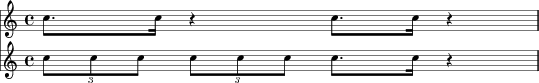
\includegraphics[width=12cm]{images/reggae.png}
\label{fig:reggae_rhythm}
\end{center}
\end{figure}

Suponiendo que el valor elegido para el per'iodo $p$ es el de $4$ negras, 

\subsection{El proceso generativo}

\subsection{Sobre la generaci\'on de r\'itmicas no vistas previamente}
Una propiedad deseable que cualquier modelo propuesto en este trabajo, en particular el reci'en descripto, es que sea capaz de generar nuevo material, distinto al de entrenamiento
pero relacionado. En este caso, el nuevo material ser'ia r'itmica \emph{nueva}, y la relaci'on con la r'itmica de entrenamiento, es que el acento m'etrico inferido sea el mismo
que la r'itmica utilizada para el entrenamiento. A continuaci'on se exhibe un ejemplo que muestra de que forma este modelo permitir'ia generar nueva r'itmica que respete 
los acentos m'etricos.

\comment{relacionar esto con lo de contexto horizontal definido en \ref{subsec_tension}}

\subsection{El valor del per\'iodo $p$}
\comment{Primer aprouch: tratar de inferir el acento metrico y construir un algoritmo que dado un mapping de acentos metricos encuentre el periodo,
       Segundo aprouch: usar el compas.
       Mencionar problemas de ambas aproximaciones}

\subsection{Generando motivos r\'itmicos}
\comment{aca voy a explicar como hacer lo de dirichlet process para generar un motivo}


%
%\subsection{El modelo}
%
%
%
%
%
%
%
%
%
%
%
%
%
%
%
%El prop'osito de este modelo es permitir trabajar con la componente temporal de la m'usica por separado del resto, 
%de modo que s'olo se trabajar'a con la relaci'on entre las duraciones de las distintas notas que
%aparecen en la pieza de entrenamiento, quedando fuera del modelo tanto la altura como la falta de sonido (silencio).
%
%
%    
%
%
%La primer relaci'on, o al menos la m'as directa, entre la duraci'on de las notas y la escucha musical es el ac'ento 
%m'etrico. La estructura m'etrica es una caracter'istica importante dentro de la musica tonal, y ser'ia deseable que el modelo construido, de alguna forma la 
%respete. 
%Supongamos por un momento que es posible realizar un algoritmo que permita inferir el acento m'etrico de cada mom Esta caracterizaci'on del tiempo permitir'ia 
